\documentclass{beamer}


\usepackage{amsmath}
\usepackage[style=alphabetic,url=true]{biblatex}
\usepackage{environ}
\usepackage{geometry}
\usepackage{graphicx}
\usepackage{tikz}
\usepackage[T2A]{fontenc}
\usepackage[utf8]{inputenc}
\usepackage[cache=false]{minted}
\usepackage{amsmath}
\usepackage{amsfonts}
\usepackage{amssymb}
\usepackage{calrsfs}


% \usetheme{Bergen}

\usecolortheme{beaver}

\setbeamertemplate{itemize item}[circle]
\setbeamertemplate{itemize subitem}{--}
\addtobeamertemplate{navigation symbols}{}{
  \usebeamerfont{footline}%
  \usebeamercolor[fg]{footline}%
  \hspace{1em}%
  \insertframenumber/\inserttotalframenumber
}
\graphicspath{ {./graphics/} }
\setminted[Python]{
  fontsize=\tiny
}
\BeforeBeginEnvironment{minted}{\medskip}
\AfterEndEnvironment{minted}{\medskip}
\usetikzlibrary{matrix}
\tikzset{
  stack/.style={
    matrix of nodes,
    nodes={
      fill=lightgray,draw,text=black,font=\sffamily\bfseries,
      text height=11pt,text depth=3pt,baseline=center, minimum width=1cm
    },
    column sep=-\pgflinewidth/2
  }
}

\title{
  Біткоїн та криптовалютні технології \\
  Лекція 5: транзакції
}

\author{Юрій Жикін}
\date{6 березня, 2025}

\begin{document}

\frame{\titlepage}

\begin{frame}
  \frametitle{Структура транзакції}
  \begin{itemize}
  \item \textbf{Транзакція}
    \begin{itemize}
    \item \textbf{входи} (список структур \textbf{Транзакційний вхід})
    \item \textbf{виходи} (список структур \textbf{Транзакційний вихід})
    \end{itemize}
  \item \textbf{Транзакійний вхід}
    \begin{itemize}
    \item \textbf{ідентифікатор попередньої транзакції}
    \item \textbf{індекс попереднього виходу} (ціле число)
    \item \textbf{програма-відмикання}
    \end{itemize}
  \item \textbf{Транзакційний вихід}
    \begin{itemize}
    \item \textbf{кількість} (ціле число)
    \item \textbf{програма-замикання}
    \end{itemize}
  \end{itemize}
\end{frame}

\begin{frame}[fragile]
  \frametitle{Передача власності над біткоїном 1/2}
  \begin{itemize}
  \item Невикористані транзакційні виходи (\textbf{UTXO}) - це записи про
    володіння ``шматками'' біткоїна: певними кількостями \textbf{сатоші},
    прив'язаними до власника за допомогою програми-замикання.
  \item Транзакції передають власність над ``шматками'' біткоїна,
    \textit{знищуючи} ці ``шматки'' (посилаючись на відповідні
    \textit{невикористані виходи} через \textit{входи}, що відмикають
    програми-замикання), та створюючи нові \textit{невикористані виходи}.
  \item Сукупність всіх \textit{невикористаних транзакційних виходів}, які
    існують в даний момент часу - це весь біткоїн, який існує в системі.
  \end{itemize}
\end{frame}

\begin{frame}[fragile]
  \frametitle{Передача власності над біткоїном 2/2}
  \begin{center}
    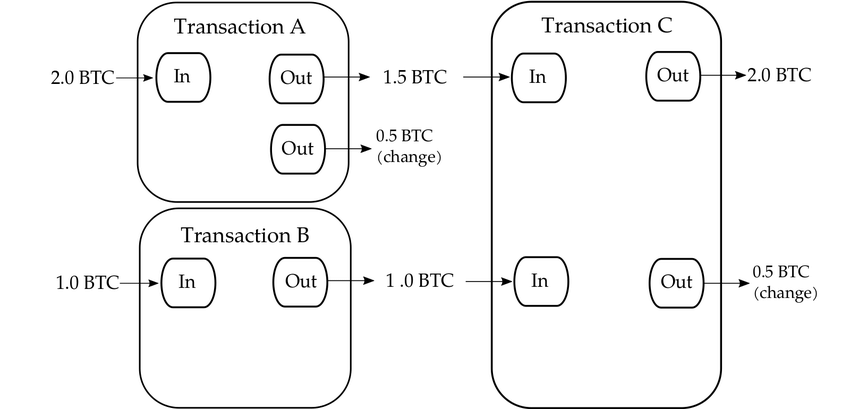
\includegraphics[width=0.8\textwidth]{transactions}
  \end{center}
\end{frame}

\begin{frame}[fragile]
  \frametitle{Валідація транзакцій}
  \begin{enumerate}
  \item \textbf{Перевірка повторного використання}: перевірка, чи виходи, на які
    посилаються входи даної транзакції, ще не були використані.
  \item \textbf{Перевірка інфляції}: перевірка, чи дана транзакція не створює
    нових біткоїнів.
  \item \textbf{Валідація контрактів}: виконання скриптів-відмикань та
    скриптів-замикань.
  \end{enumerate}
\end{frame}

\begin{frame}[fragile]
  \frametitle{Біткоїн Скрипт}
  \begin{itemize}
  \item \textbf{Біткоїн Скрипт}, або просто \textbf{Скрипт} - це
    \textbf{стекова} \textbf{Forth-подібна} \textbf{Тюрінг-неповна} мова програмування
    для формулювання логіки замикання/відмикання транзакційних виходів.
  \item Скрипт дозволяє формулювати довільні умови використання кожного окремого
    ``шматка'' біткоїна.
  \item Система \textit{доказу виконаної роботи} реалізує децентралізовану
    перевірку повторного використання, а система \textit{скриптування} -
    програмованість (``розумні контракти'').
  \end{itemize}
\end{frame}

\begin{frame}[fragile]
  \frametitle{Стекові мови програмування}
  \begin{itemize}
  \item \textbf{Стекове програмування} - це парадигма програмування, яка
    базується на моделі \textbf{стекової машини} для передачі параметрів.
  \item Приклад:
    \begin{enumerate}
    \item
      \begin{tabular}{rl}
        Програма &\mintinline[bgcolor=lightgray]{Lisp}{3 5 add 3 mul;} \\
        Дані &\mintinline[bgcolor=lightgray]{Lisp}{;} \\
      \end{tabular}
    \item
      \begin{tabular}{rl}
        Програма &\mintinline[bgcolor=lightgray]{Lisp}{5 add 3 mul;} \\
        Дані &\mintinline[bgcolor=lightgray]{Lisp}{3;} \\
      \end{tabular}
    \item
      \begin{tabular}{rl}
        Програма &\mintinline[bgcolor=lightgray]{Lisp}{add 3 mul;} \\
        Дані &\mintinline[bgcolor=lightgray]{Lisp}{5 3;} \\
      \end{tabular}
    \item
      \begin{tabular}{rl}
        Програма &\mintinline[bgcolor=lightgray]{Lisp}{3 mul;} \\
        Дані &\mintinline[bgcolor=lightgray]{Lisp}{8;} \\
      \end{tabular}
    \item
      \begin{tabular}{rl}
        Програма &\mintinline[bgcolor=lightgray]{Lisp}{mul;} \\
        Дані &\mintinline[bgcolor=lightgray]{Lisp}{3 8;} \\
      \end{tabular}
    \item
      \begin{tabular}{rl}
        Програма &\mintinline[bgcolor=lightgray]{Lisp}{;} \\
        Дані &\mintinline[bgcolor=lightgray]{Lisp}{24;} \\
      \end{tabular}
    \end{enumerate}
  \end{itemize}
\end{frame}

\begin{frame}[fragile]
  \frametitle{Тюрінг-неповнота}
  \begin{itemize}
  \item \textit{Скрипт} - це \textit{навмисно} Тюрінг-неповна мова
    програмування.
  \item У Скрипті відсутній один з основних інструментів сучасних мов
    програмування: \textbf{цикл}.
  \item Скрипти у транзакціях виконуються кожною повноцінною нодою в мережі, і
    тому цикли могли б використовуватись як засіб завантаження мережі
    (здійснення DoS-атак).
  \item Програми з циклами значно гірше піддаються статичному аналізу (тобто
    аналізу, який ``розглядає'' програму, але не виконує її).
  \item Мережа Етереум використовує Тюрінг-повну мову \textbf{Solidity}, що є
    безпосереднім чинником найбільших безпекових інцидентів за весь час
    існування Етереум-мережі.
  \end{itemize}
\end{frame}

\begin{frame}[fragile]
  \frametitle{Операції у Біткоїн Скрипті 1/3}
  \begin{itemize}
  \item \textit{Інтерпретатор скрипта} складається зі стеку команд та стеку даних.
  \item Для кожного \textit{входу} транзакції, спочатку виконується його
    програма-відмикання, а отриманий стек даних використовується для подальшого
    виконання програми-замикання відповідного \textit{виходу}:
    \begin{itemize}
    \item створюємо порожній стек $Stack_0 = Stack_{empty}$
    \item виконуємо програма-відмикання входу на стеку $Stack_0$:
      $$Stack_1 = Execute(Script_{Unlock}, Stack_0)$$
    \item виконуємо програма-замикання відповідного виходу на стеку $Stack_1$:
      $$Stack_2 = Execute(Script_{Lock}, Stack_1)$$
    \item перевіряємо, чи верхній елемент стеку $Stack_2$ - не $False$.
    \end{itemize}
  \end{itemize}
\end{frame}

\begin{frame}[fragile]
  \frametitle{Операції у Біткоїн Скрипті 2/3}
  \begin{itemize}
  \item Значення на стеку даних - це послідовності байтів, але вони можуть
    інтерпретуватись, як числа, коли це необхідно.
  \item Значення $False$ представляється числом 0, яке в свою чергу
    представляється порожньою послідовністю байтів, бо послідовністю з одного
    байта $[0x80]$.
  \item Будь-яке значення, що не є $False$, вважається значенням $True$.
  \item Будь-яка послідовність, крім $\{[], [0x80]\}$ на верхівці стека даних
    після виконання скриптів означає, що контракт даного ``шматка'' біткоїна є
    правильним.
  \item Виконання скрипта також може завершитись помилкою, що прирівнються до
    значення $False$.
  \end{itemize}
\end{frame}

\begin{frame}[fragile]
  \frametitle{Операції у Біткоїн Скрипті 3/3}
  \begin{itemize}
  \item \textbf{константи} - розміщення даних у стеку
  \item \textbf{бітова логіка та арифметика}
  \item \textbf{маніпуляція стеком} - викидання, копіювання, перестановка
    елементів стека
  \item \textbf{контроль виконання} - умовні операції, а також
    \begin{itemize}
    \item \mintinline{Python}{OP_VERIFY} - помилка, якщо на верхівці стека -
      не $True$
    \item \mintinline{Python}{OP_RETURN} - завжди помилка (використовується
      для розміщення довільних даних всередині транзакції: зображень, тощо)
    \end{itemize}
  \item \textbf{криптографія} - криптографічні операції (хеш-функції)
    \begin{itemize}
    \item \mintinline{Python}{OP_CHECKSIG} - перевірка підпису для заданого
      публічного ключа
    \item \mintinline{Python}{OP_CHECKMULTISIG} - перевірка декількох підписів
      для декількох публічних ключів (контракти типу ``$N$ з $M$ власників'')
    \end{itemize}
  \item \textbf{блокування} - перевірка умов блокування транзакцій
  \end{itemize}
\end{frame}

\begin{frame}[fragile]
  \frametitle{Стандартні Скрипти-програми 1/4}
  \begin{itemize}
  \item \textbf{P2PKH} - pay-to-pubkey-hash (платіж за хешем публічного ключа)
    \break
    \begin{tabular}{rl}
      Замикання &\tiny\mintinline[bgcolor=lightgray]{Lisp}{OP_DUP OP_HASH160 <pubKeyHash> OP_EQUALVERIFY OP_CHECKSIG;} \\
      Відмикання &\tiny\mintinline[bgcolor=lightgray]{Lisp}{<sig> <pubKey>;} \\
    \end{tabular}
  \item Виконання P2PKH-скриптів
    \begin{enumerate}
    \item
      \begin{tabular}{rl}
        Програма &\tiny\mintinline[bgcolor=lightgray]{Lisp}{<sig> <pubKey>;} \\
        Дані &\tiny\mintinline[bgcolor=lightgray]{Lisp}{;} \\
      \end{tabular}
    \item
      \begin{tabular}{rl}
        Програма &\tiny\mintinline[bgcolor=lightgray]{Lisp}{<pubKey>;} \\
        Дані &\tiny\mintinline[bgcolor=lightgray]{Lisp}{<sig>;} \\
      \end{tabular}
    \item
      \begin{tabular}{rl}
        Програма &\tiny\mintinline[bgcolor=lightgray]{Lisp}{;} \\
        Дані &\tiny\mintinline[bgcolor=lightgray]{Lisp}{<pubKey> <sig>;} \\
      \end{tabular}
    \end{enumerate}
  \end{itemize}
\end{frame}

\begin{frame}[fragile]
  \frametitle{Стандартні Скрипт-програми 2/4}
  \begin{itemize}
  \item Виконання P2PKH-програми
    \begin{enumerate}
    \item
      \begin{tabular}{rl}
        Програма &\tiny\mintinline[bgcolor=lightgray]{Lisp}{OP_DUP OP_HASH160 <pubKeyHash> OP_EQUALVERIFY OP_CHECKSIG;} \\
        Дані &\tiny\mintinline[bgcolor=lightgray]{Lisp}{<pubKey> <sig>;} \\
      \end{tabular}
    \item
      \begin{tabular}{rl}
        Програма &\tiny\mintinline[bgcolor=lightgray]{Lisp}{OP_HASH160 <pubKeyHash> OP_EQUALVERIFY OP_CHECKSIG;} \\
        Дані &\tiny\mintinline[bgcolor=lightgray]{Lisp}{<pubKey> <pubKey> <sig>;} \\
      \end{tabular}
    \item
      \begin{tabular}{rl}
        Програма &\tiny\mintinline[bgcolor=lightgray]{Lisp}{<pubKeyHash> OP_EQUALVERIFY OP_CHECKSIG;} \\
        Дані &\tiny\mintinline[bgcolor=lightgray]{Lisp}{<pubKeyHash> <pubKey> <sig>;} \\
      \end{tabular}
    \item
      \begin{tabular}{rl}
        Програма &\tiny\mintinline[bgcolor=lightgray]{Lisp}{OP_EQUALVERIFY OP_CHECKSIG;} \\
        Дані &\tiny\mintinline[bgcolor=lightgray]{Lisp}{<pubKeyHash> <pubKeyHash> <pubKey> <sig>;} \\
      \end{tabular}
    \item
      \begin{tabular}{rl}
        Програма &\tiny\mintinline[bgcolor=lightgray]{Lisp}{OP_CHECKSIG;} \\
        Дані &\tiny\mintinline[bgcolor=lightgray]{Lisp}{<pubKey> <sig>;} \\
      \end{tabular}
    \item
      \begin{tabular}{rl}
        Програма &\tiny\mintinline[bgcolor=lightgray]{Lisp}{;} \\
        Дані &\tiny\mintinline[bgcolor=lightgray]{Lisp}{True;} \\
      \end{tabular}
    \end{enumerate}
  \end{itemize}
\end{frame}

\begin{frame}[fragile]
  \frametitle{Стандартні Скрипт-програми 3/4}
  \begin{itemize}
  \item \textbf{P2PK} - pay-to-pubkey (платіж за публічним ключем, більше не
    використовується, бо публічний ключ потрапляє в ланцюг блоків занадто рано)
    \break
    \begin{tabular}{rl}
      Замикання &\tiny\mintinline[bgcolor=lightgray]{Lisp}{<pubKey> OP_CHECKSIG;} \\
      Відмикання &\tiny\mintinline[bgcolor=lightgray]{Lisp}{<sig>;} \\
    \end{tabular}
  \item \textbf{P2MS} - багатопідписні транзакції (``$M$ з $N$ власників'')
    \break
    \begin{tabular}{rl}
      Замикання &\tiny\mintinline[bgcolor=lightgray]{Lisp}{<M> <pk1> ... <pkN> <N> OP_CHECKMULTISIG;} \\
      Відмикання &\tiny\mintinline[bgcolor=lightgray]{Lisp}{OP_0 <sig1> ... <sigM>;} \\
    \end{tabular}
  \item \textbf{P2SH} - pay-to-script-hash (платіж за хешем скрипта) - зміна
    протоколу, впроваджена у 2012 році, яка дозволила створювати довільні
    скрипти-замикання, які при цьому мають фіксований розмір та визначену адресу
    \break
    \begin{tabular}{rl}
      Замикання &\tiny\mintinline[bgcolor=lightgray]{Lisp}{OP_HASH160 <scriptHash> OP_EQUAL;} \\
      Відмикання &\tiny\mintinline[bgcolor=lightgray]{Lisp}{<customLockScript...> <serializedRedeemScript>;} \\
    \end{tabular}
  \end{itemize}
\end{frame}

\begin{frame}[fragile]
  \frametitle{Стандартні Скрипт-програми 4/4}
  \begin{itemize}
  \item \textbf{P2SH} потребував зміни правил виконання \textit{Скрита} за
    допомогою \textit{м'якого розгалуження}:
    \begin{itemize}
    \item виконуємо скрипт-відмикання, отримуємо
      \mintinline{Python}{<serializedRedeemScript>} на верхівці стека
    \item виконуємо скрипт-замикання, перевіряючи, що закодований скрипт 
      \mintinline{Python}{<serializedRedeemScript>} відповідає хешу
      \mintinline{Python}{<scriptHash>}
    \item учасники мережі з \textbf{старою} версією протоколу вважають, що
      транзакція правильна
    \item учасники мережі з \textbf{новою} версією протоколу продовжують
      перевірку: декодують скрипт \mintinline{Python}{<serializedRedeemScript>}
      і виконують його, так ніби це справжній скрипт-замикання
    \end{itemize}
  \end{itemize}
\end{frame}

\begin{frame}[fragile]
  \frametitle{Види розгалужень у мережі}
  \begin{itemize}
  \item \textbf{М'яке розгалуження} (англ. \textit{softfork}) робить правила
    \textbf{більш строгими}, тобто старі учасники зі старими правилами вважають
    нові дані завжди правильними, а нові учасники здійснюють додаткові перевірки
  \item \textbf{Жорстке розгалуження} (англ. \textit{hardfork}) робить правила
    \textbf{менш строгими}, тобто старі учасники відкинуть дані, як неправильні,
    але нові учасники вважають ці дані правильними, що розділяє мережу на дві
    частини, і тому всі учасники повинні оновити набір правил, для того, щоб
    мережа продовжила працювати
  \item \textbf{Жорстке розгалуження} ``викидає'' старих учасників мережі з
    протоколу
  \end{itemize}
\end{frame}

\begin{frame}[fragile]
  \frametitle{Нестандартні програми-замикання}
  \begin{itemize}
  \item \textbf{Задача SHA256} - ``шматок'' біткоїна може використати будь-хто,
    хто надасть таку послідовність байтів $s$, що $h = SHA256(s)$
    \break
    \begin{tabular}{rl}
      Замикання &\tiny\mintinline[bgcolor=lightgray]{Lisp}{OP_HASH256 <h> OP_EQUAL;} \\
      Відмикання &\tiny\mintinline[bgcolor=lightgray]{Lisp}{<s>;} \\
    \end{tabular}
  \item \textbf{Задача колізії SHA1} - створена Пітером Тодом в 2013 році для
    заохочення пошуку колізій для хеш-функції SHA1, яка вже на той час вважалась
    небезпечною; 2.48 біткоїнів винагороди хтось забрав у 2017 році:
    \break
    \begin{tabular}{rl}
      Замикання &\tiny\mintinline[bgcolor=lightgray]{Lisp}{OP_2DUP OP_EQUAL OP_NOT OP_VERIFY OP_SHA1 OP_SWAP OP_SHA1 OP_EQUAL;} \\
      Відмикання &\tiny\mintinline[bgcolor=lightgray]{Lisp}{<preimage1> <preimage2>;} \\
    \end{tabular}
  \end{itemize}
\end{frame}

\begin{frame}[fragile]
  \frametitle{Біткоїн-адреси 1/2}
  \begin{itemize}
  \item Для \textit{стандартних} виходів транзакцій (тобто виходів, що мають
    \textit{стандартну} програму-замикання), існують визначені формати ``адрес''.    
  \item Біткоїн-адреси - це невеликі (порівняно) ідентифікатори, які однозначно
    описують скрипт-замикання і використовуються замість цілого скрипта для
    отримання транзакції
    \begin{itemize}
    \item для \textit{P2PKH}, це \mintinline{Python}{<pubKeyHash>}:
      $$A_{P2PKH} = Encode_{Base58Check}(HASH160(pubkey))$$
    \item для \textit{P2SH}, це \mintinline{Python}{<scriptHash>}:
      $$A_{P2SH} = Encode_{Base58Check}(HASH160(redeemscript))$$
    \end{itemize}
  \end{itemize}
\end{frame}

\begin{frame}[fragile]
  \frametitle{Біткоїн-адреси 2/2}
  \begin{itemize}
  \item Для того, щоб уникати неоднозначностей і зменшити ймовірність помилок,
    традиційні Біткоїн-адреси використовують спеціальне кодування
    \textbf{Base58Check}:
    $$Base58Check(t, s) = Base58(t + s + HASH256(t + s)[0:4])$$
  \item \textbf{Base58}-кодування схоже на 64-кове кодування (\textbf{base64}),
    але навмисне не використовує символи, які можна легко сплутати з іншими: 0,
    O, I, and l.
  \item Значення $t$ використовується, щоб ідентифікувати тип інформації, яка
    кодується:
    \break
    \break
    \tiny
    \begin{tabular}{cccl}
      0 & 1 & \mintinline{Python}{"18vnsHEtfTZgaJD6Sv7QTpo2nwxkFxJgrp"} & P2PKH-адреси \\
      5 & 3 & \mintinline{Python}{"38Rctgcqj3cFhfGK7ynpWZQZgCTVuCoNFu"} & P2SH-адреси \\
      111 & m or n & \mintinline{Python}{"mkHS9ne12qx9pS9VojpwU5xtRd4T7X7ZUt"} & P2PKH-адреси у тестовій мережі \\
      196 & 2 & \mintinline{Python}{"2N4DTeBWDF9yaF9TJVGcgcZDM7EQtsGwFjX"} & P2SH-адреси у тестовій мережі \\
    \end{tabular}
  \end{itemize}
\end{frame}

\begin{frame}[fragile]
  \frametitle{Біткоїн-гаманець 1/2}
  \begin{itemize}
  \item В загальному випадку, Біткоїн-гаманець - це будь-яка інформація,
    використовуючи яку, можна створити програму-відмикання для деякого
    \textit{невикористаного транзакційного виходу}.
  \item Типовий Біткоїн-гаманець - це програмне забезпечення, що зберігає
    криптографічні ключі і вміє розбирати та створювати станданртні транзакції.
  \item Коли користувач хоче отримати біткоїн, Біткоїн-гаманець генерує нову
    пару криптографічних ключів $(p_i, P_i)$ і обчислює нову P2PKH-адресу $A_i$
    наступним чином
    $$A_i = Encode_{Base58Check}(HASH160(P_i))$$
  \end{itemize}
\end{frame}

\begin{frame}[fragile]
  \frametitle{Біткоїн-гаманець 2/2}
  \begin{itemize}
  \item Цю адресу отримувач передає надсилачеві.
  \item Гаманець надсилача обчислює $H = Decode_{Base58Check}(A_i)$ і створює
    транзакцію з виходом з вказаною кількістю біткоїна тапрограмою-замиканням,
    що містить вказаний хеш $H$
    \begin{center}
      \tiny\mintinline[bgcolor=lightgray]{Lisp}{OP_DUP OP_HASH160 <H> OP_EQUALVERIFY OP_CHECKSIG;}
    \end{center}
  \item Гаманець надсилача знаходить у своєму сховищі криптографічні ключі, що
    відповідають \textit{виходам}, які він ``витрачає'', і обчислює відповідні
    підписи, щоб створити відповідні програми-відмикання.
  \item Заповнена транзакція публікується, потрапляє у блок і підтверджується.
  \item Тепер отримувач має право власності над створеним \textit{виходом} і
    може аналогічним чином використати його.
  \end{itemize}
\end{frame}

\begin{frame}
  \frametitle{Кінець}
  \begin{center}
    Дякую за увагу!
  \end{center}
\end{frame}

\end{document}

%%% Local Variables:
%%% mode: latex
%%% TeX-master: t
%%% End:
